\documentclass[letterpaper,12pt]{scrartcl}
\usepackage{epsfig,latexsym,amsmath,amssymb,epic,eepic,psfrag,subfigure,float,euscript,array}
\usepackage[latin1]{inputenc}
\usepackage[margin=24mm]{geometry}
\usepackage{enumitem}
\usepackage{tikz,pgf,pgfplots}
\usepgfplotslibrary{fillbetween}
\usepgfplotslibrary{groupplots}
\usetikzlibrary{decorations, arrows}

\usepackage[amssymb]{SIunits}

\newenvironment{exercise}[1][Problem]{\begin{trivlist} \item[\hskip
    \labelsep {\stepcounter{exerctr}\bfseries #1
      \arabic{exerctr}}]}{\end{trivlist}\vspace{10mm}}

\newcounter{exerctr}
\newcounter{abcctr}[exerctr]

\newcommand{\abc}{\noindent\vspace{1mm}\\ {\bf
    \stepcounter{abcctr}(\alph{abcctr})\ }}
\newcommand{\bbm}{\begin{bmatrix}}
\newcommand{\ebm}{\end{bmatrix}}
\newcommand{\point}[1]{\hfill {\bf (#1p)}\\ \vspace{-5mm}}
\newcommand{\ctrb}{\EuScript{S}}
\newcommand{\Lap}{\mathcal{L}}
\newcommand{\obsv}{\EuScript{O}}
\newcommand{\realdel}{\text{Re}}
\newcommand{\imagdel}{\text{Im}}
\newcommand{\bC}{\mathbb{C}}
\newcommand{\bR}{\mathbb{R}}
\newcommand{\bmpv}{\begin{minipage}[t]}
\newcommand{\bmps}{\begin{minipage}[t]{45mm}}
\newcommand{\bmpm}{\begin{minipage}[t]{90mm}}
\newcommand{\bmpl}{\begin{minipage}[t]{\textwidth}}
\newcommand{\emp}{\end{minipage}}
\newcommand{\mexp}[1]{\ensuremath{\mathrm{e}^{#1}}}
\newcommand*{\laplaceinv}[1]{\ensuremath{\mathcal{L}^{-1} \left\{#1\right\}}}
\newcommand*{\ztrf}[1]{\ensuremath{\mathcal{Z} \left\{#1\right\}}}

\newcommand{\AxisRotator}[1][rotate=0]{%
    \tikz [x=0.2cm,y=0.60cm,line width=.1ex,-stealth,#1] \draw (0,0) arc (-150:150:1 and 1);%
}

\newcommand{\shift}{\ensuremath{\operatorname{q}}}
%\addtolength{\topmargin}{-1cm}
%\textheight 22.5cm
%\oddsidemargin 1.3cm
%\evensidemargin 1.3cm

\makeatletter
\newcommand*{\rom}[1]{\expandafter\@slowromancap\romannumeral #1@}
\makeatother

\newcommand*\circled[1]{\tikz[baseline=(char.base)]{
            \node[shape=circle,draw,inner sep=2pt] (char) {#1};}}


\pgfplotstableread[col sep=comma]{BLDC-step-partial2-fall18.dta}\inputtable
\pgfplotstableread[col sep=comma]{BLDC-closed-loop-step-partial2-fall18.dta}\clsteptable
\pgfplotstableread[col sep=comma]{BLDC-closed-loop-bode-partial2-fall18.dta}\bodetable
%\pgfplotstableread[col sep=comma]{responses.dat}\outputtable

\title{Computerized Control partial exam 2 (18\%)}
\author{Kjartan Halvorsen}
\date{}

\begin{document}

\maketitle


\begin{description}
\item[Time] October 24 19:05-20.35
\item[Place] 4203
\item[Permitted aids] The single colored page with your own notes, table of Laplace transforms, calculator
\end{description}

All answers should be readable and well motivated (if nothing else is written). Solutions/motivations should be written on the provided spaces in this exam. Use the last page if more space is needed.

\begin{center}
{\Large Good luck!} \\
\end{center}

\noindent
\fbox{
\bmpl
{\bf Matricula and name:}\\
\vspace*{14mm}
\emp}


%\clearpage

%-----------------------------------------------------------------

% https://www.hindawi.com/journals/mpe/2015/879581/
\subsection*{Control of a brushless DC motor}
Consider a brushless DC (BLDC) motor with electronic speed control (ESC). Under a typical load the response of the motor is described by a pulse-transfer function $H(z)$. The load is not constant, however, and load changes are represented as an additive disturbance $v(k)$ on the output. The input signal $u(k)$ represents the desired (average) voltage over the windings of the motor, which is translated into a pulse-width-modulation signal before being sent to the ESC. The output signal $y(k)$ is the speed of the motor.
\begin{center}
  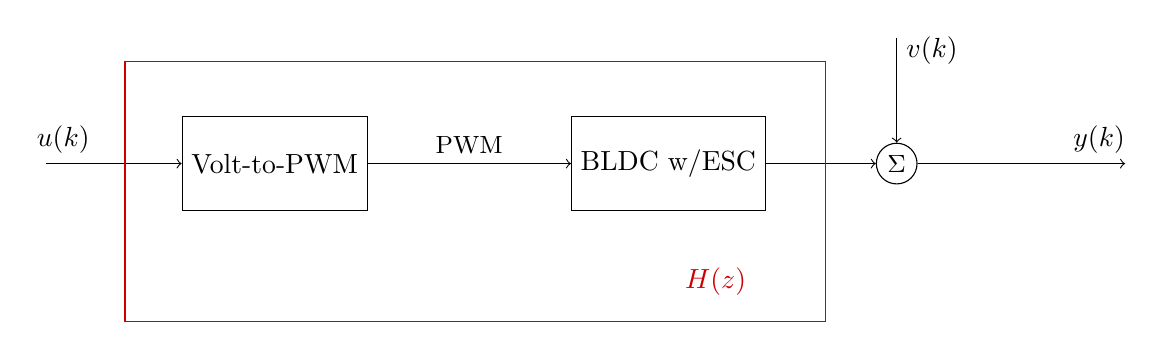
\begin{tikzpicture}[node distance = 2.9cm, block/.style={draw, minimum height=12mm, minimum width=15mm}]
    \node[coordinate] (input) {};
    \node[block, right of=input] (v2pwm) {Volt-to-PWM};
    \node[block, right of=v2pwm, node distance=5cm] (bldc) {BLDC w/ESC};
    \node[circle, draw, inner sep=2pt, right of=bldc] (sum) {\small $\Sigma$};
    \node[coordinate, right of=sum] (output) {};
    \node[coordinate, above of=sum, node distance=16mm] (dist) {};
    
    \draw[->] (dist) -- node[right, very near start] {$v(k)$} (sum);
    \draw[->] (input) -- node[above, very near start] {$u(k)$} (v2pwm);
    \draw[->] (v2pwm) -- node[above, ] {\small PWM} (bldc);
    \draw[->] (bldc) -- node[above, near end] {$$} (sum);
    \draw[->] (sum) -- node[above, very near end] {$y(k)$} (output);

    \draw[red!80!black] (1,-2) rectangle (9.9,1.3);
    \node[red!80!black] at (8.5, -1.5) {$H(z)$};

  \end{tikzpicture}
\end{center}

\begin{exercise}

The step response of the pulse-transfer function $H(z)$ is given in figure \ref{fig:step}. Below are four different pulse-transfer functions. Plot the poles and zeros of each of the four pulse-transfer functions in the z-plane, and determine which pulse-transfer function corresponds to the step response in figure \ref{fig:step}. \textbf{Motivate!}

%\tikzset{plttype/.style={ycomb, thick, mark=*, mark options={red!60!black}}}
\tikzset{plttype/.style={const plot, no marks, ultra thick}}
\tikzset{plttypeu/.style={const plot, no marks, thick, blue!70}}

\begin{figure}[h]
\begin{center}
\begin{tikzpicture}
\begin{axis}[
  width=15cm,
  height=5cm,
  xlabel={$k$},
  ylabel={$y(k)$ [$\times$ 1000 RPM]\\ $u(k)$ [V]},
  ylabel style={align=center, text width=8cm},
  %axis lines=middle,
  %xmin=-.5,
  %xmax=6.5,
  %ymin = -2.5, ymax = 2.5,
  %xtick = {1,2,3,4,5,6},
]

\addplot[plttype] table[x=1, y = 2] from \inputtable node [coordinate, pos=0.9, pin=-20:{$y(k)$}] {};
\addplot[plttypeu, domain=-1:24, ] {(x>0)} node [coordinate, pos=0.9, pin=20:{$u(k)$}] {};
\end{axis}
\end{tikzpicture}
\caption{Step-response of $H(z)$.}
\label{fig:step}
\end{center}
\end{figure}

\begin{tabular}{ll}
$H_1(z) = \frac{0.66(z+1.13)(z+0.08)}{z(z-0.73)(z-0.01 + 0.1j)(z-0.01 - 0.1j)} $ &
$H_2(z) = \frac{0.66(z+1.13)(z+0.08)}{z(z-0.99)} $\\[4mm]
$H_3(z) = \frac{0.66(z+1.13)(z+0.08)}{z(z-0.73)(z-0.8 + 0.6j)(z-0.8 - 0.6j)} $ &
$H_4(z) = \frac{0.66(z+1.13)(z+0.08)}{z^2(z-0.73)(z-1.03)}$
\end{tabular}

\begin{center}
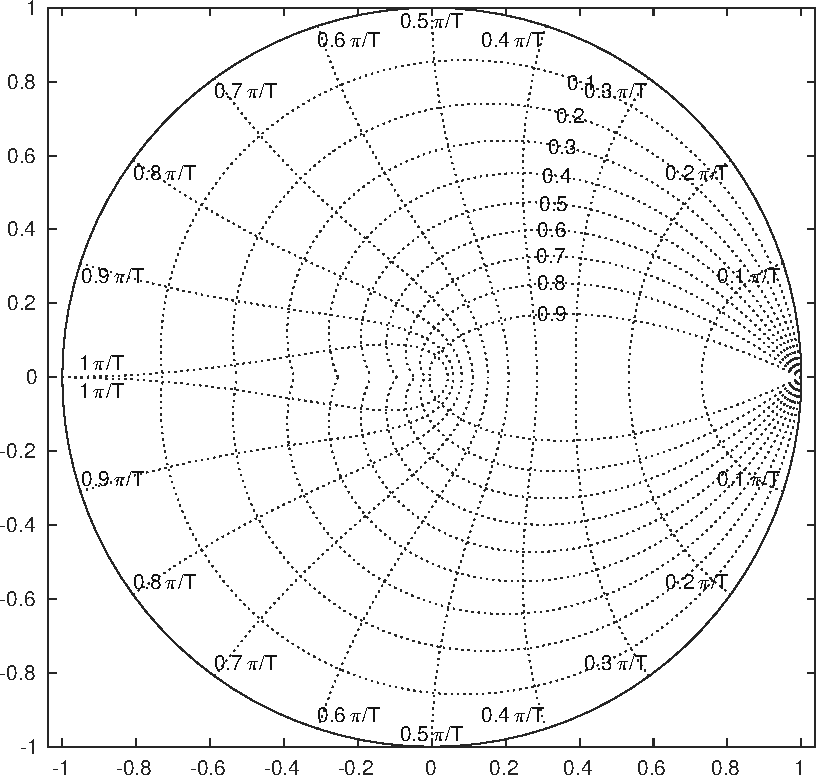
\includegraphics[width=0.7\linewidth]{../../figures/zgrid-crop}
\end{center}

\noindent
\fbox{
\bmpl
{\bf Motivation:}\\
\vspace*{70mm}
\emp}
\end{exercise}


\begin{exercise}
A two-degree-of-freedom \textbf{incremental} controller
is sought for the BLDC. See figure \ref{fig:block}. The specifications on the control system states that the desired poles of the closed-loop pulse-transfer function from the command signal $u_c(k)$ to the output $y(k)$ should all be in $z=0.6$, and that all observer poles should be in the origin, $z=0$. 

\begin{figure}[h]
\begin{center}
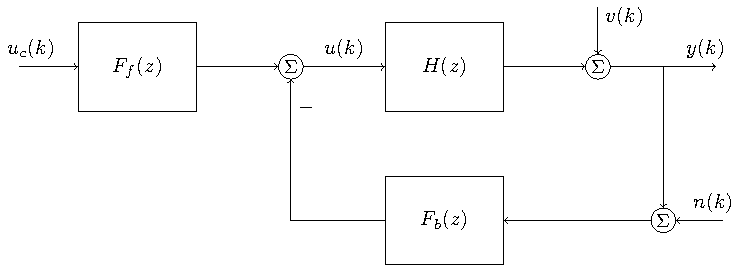
\includegraphics[width=0.7\linewidth]{../../figures/2dof-block-complete}
\end{center}
\caption{Two-degree-of-freedom control system.}
\label{fig:block}
\end{figure}

\abc Write down the Diophantine equation. You don't have to multiply the polynomials. Determine the order of the controller, and write out the polynomials of the left-hand side of the Diophantine equation, i.e.~the polynomials $A(z)$, $B(z)$, $S(z)$ and $R(z)$. Show that the Diophantine equation leads to a number of equations that equals the number of unknown controller-parameters.

\noindent
\fbox{
\bmpl
{\bf Calculations:}\\
\vspace*{125mm}
\emp}


\abc Choose an observer polynomial $A_o(z)$, and determine the polynomial $A_c(z)$ in the factorization  $A_{cl}(z) = A_c(z)A_o(z)$ of the right-hand side of the Diophantine equation. \textbf{Motivate!}

\noindent
\fbox{
\bmpl
{\bf Answer and motivation:}\\
\vspace*{90mm}
\emp}

\end{exercise}

\begin{exercise}

The closed-loop pulse-transfer function from disturbance $v(k)$ to output $y(k)$ for the two-degree-of-freedom control system given in the block diagram (figure \ref{fig:block}) is given by
\begin{equation}
 H_{v,1}(z) = \frac{1}{1 + H(z)F_b(z)}.
 \label{eq:Hv}
\end{equation}
When implementing the controller it was observed that the measured continuous-time output signal $y(t)$ was quite noisy, and an anti-aliasing filter was included in order to low-pass filter $y(t)$ before sampling. The discrete-time closed-loop pulse-transfer of the system with anti-aliasing filter is (approximately)
\begin{equation}
 H_{v,2}(z) = \frac{1}{1 + H(z)F_b(z)\cdot\frac{1}{z^2}}.
 \label{eq:Hv2}
\end{equation}

\abc
Figure \ref{fig:clstep} shows the step responses of $H_{v,1}(z)$ and $H_{v,2}(z)$, respectively. Which is which? Motivate. Describe also three interesting details in the step responses and explain (in 3-5 sentences) the reason why this happens.
 
\tikzset{plttype1/.style={const plot, no marks, ultra thick, orange!80!black}}
\tikzset{plttype2/.style={const plot, no marks, ultra thick, green!60!black}}
\tikzset{plttypeu/.style={const plot, no marks, thick, blue!70}}

\begin{figure}[h]
\begin{center}
\begin{tikzpicture}
\begin{axis}[
  width=15cm,
  height=5cm,
  xlabel={$k$},
  ylabel={$y(k)$},
  ylabel style={align=center, text width=8cm},
  %axis lines=middle,
  xmin=-.5,
  xmax=60,
  grid=both,
  %ymin = -2.5, ymax = 2.5,
  %xtick = {1,2,3,4,5,6},
]

\addplot[plttype1] table[x=1, y = 2] from \clsteptable ;
\addplot[plttype2] table[x=1, y = 3] from \clsteptable ; %node [coordinate, pos=0.9, pin=20:{$y(k)$}] {};
%\addplot[thin, dashed, no marks, domain=-1:60, ] {0};
\end{axis}
\end{tikzpicture}
\caption{Responses of closed-loop systems $H_{v,1}(z)$ and $H_{v,2}(z)$, respectively, to a step in disturbance $v(k)$.}
\label{fig:clstep}
\end{center}
\end{figure}

\noindent
\fbox{
\bmpl
{\bf Answer:}\\
\vspace*{80mm}
\emp}

\abc [Bonus question worth 5p] Note that one of the step-responses in figure \ref{fig:clstep} shows damped oscillations. \textbf{What is the period of the oscillations (in terms of the sampling period)?} Look carefully at the Bode plot below, which corresponds to the system with oscillatory reponse (only the magnitude plot in the frequency band 0.1 to \unit{10}{\rad\per\second} is shown). \textbf{What is the sampling period in seconds?}
\begin{center}
\begin{tikzpicture}
  \begin{loglogaxis} [
      xlabel={$\omega$ [rad/s]},
      ylabel=$|H_v(i\omega)|$,
      width=13cm,
      height=6cm,
      grid=both,
      every major grid/.style={red, opacity=0.5},
      %ytick={0.5, 2},
      %yticklabels={$\frac{J\omega_0}{k_d2}$, $\frac{2J\omega_0}{k_d}$},
      %xticklabel=\empty,
      %ymin=0.2, ymax=6,
      xmin=0.1, xmax=10,
      %legend entries={Bessel filter, Delay of one},
      %legend pos={south west},
  ]
    \addplot [thick,black, no marks, ] table [x=0, y=1 ] from \bodetable;
  \end{loglogaxis}
\end{tikzpicture}
\end{center}  

\noindent
\fbox{
\bmpl
{\bf Calculations and motivation:}\\
\vspace*{60mm}
\emp}

\end{exercise}

\cleardoublepage
%\end{document}

\section*{Solutions}
\setcounter{exerctr}{0} 

\begin{exercise}

The below pole-zero map is obtained.
\begin{center}
  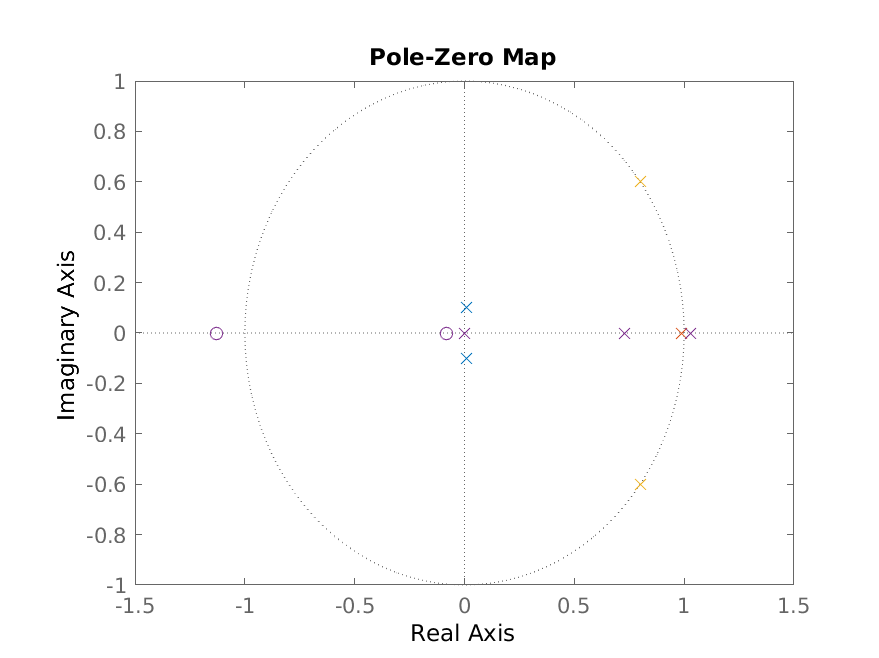
\includegraphics[width=0.7\linewidth]{BLDC-pzmap}
\end{center}  

In the step response of figure \ref{fig:step} it can be observed that the response starts at $k=2$. This means that the pole-excess (the difference between the number of poles and the number of zeros) must be 2. The response has no overshoot, and no oscillations. The half-time (the time it takes for the response to half the distance to the final value) is about $T_h=3$, which indicates that the system should have a dominating pole in approximately $p^3 = 0.5$ which gives $p=(0.5)^{\frac{1}{3}}=0.79$. The system  $H_1(z) = \frac{0.66(z+1.13)(z+0.08)}{z(z-0.73)(z-0.01 + 0.1j)(z-0.01 - 0.1j)} $ is the only system that shows all of these characteristics. 

It is also possible to find the correct answer by eliminating the other alternatives. System $H_2(z)$ has a pole-excess of 0, so the response should start at $k=0$. System $H_3(z)$ has two poles on the unit circle, and so should show undamped oscillations. Finally, system $H_4(z)$ has an unstable pole in $z=1.03$ and so should show a diverging response. We're left with system $H_1(z)$.

\end{exercise}

\begin{exercise}
\abc 
The characteristic equation for the closed-loop system is $1+H(z)F_b(z)=0$. With $H(z)= \frac{B(z)}{A(z)}$, and $F_b(z) = \frac{S(z)}{R(z)} = \frac{S(z)}{(z-1)\bar{R}(z)}$, the characteristic equation becomes 
\[ 1 + \frac{B(z)S(z)}{A(z)(z-1)\bar{R(z)}} = \frac{A(z)(z-1)\bar{R}(z) + B(z)S(z)}{A(z)(z-1)\bar{R}(z)} = 0\,\]
which gives the characteristic equation
\[ A(z)(z-1)\bar{R}(z) + B(z)S(z) = 0,\]
and the characteristic polynomial 
\[ A(z)(z-1)\bar{R}(z) + B(z)S(z).\]
The closed-loop specifications lead to the desired characteristic polynomial 
\(A_c(z)A_o(z)\), and equating the two characteristic polynomials gives the Diophantine equation
\[ A(z)(z-1)\bar{R}(z) + B(z)S(z) = A_c(z)A_o(z).\]
The idea behind the design technique is to determine the controller polynomials $S(z)$ and $\bar{R}(z)$ so that the characteristic polynomial on the left hand side equals the desired (given) characteristic polynomial on the right hand side. 
 
The number of equations from the Diophantine equation equals the degree of the polynomials on each side of the equality sign, which is $\deg A + 1+\deg \bar{R}= 5+\deg\bar{R}$. The feedback controller has $2\deg\bar{R}+2$ unknown parameters, since the denominator has $\deg\bar{R}$ parameters and the numerator has $\deg\bar{R} + 2$ parameters (there is a coefficient $s_0$ for the term of highest power and $\deg S = \deg\bar{R} + 1$). To have the same number of equations as unknowns ($5+\deg\bar{R} = 2\deg\bar{R}+2$), we choose $\deg\bar{R}=3$. This gives the controller polynomials
\begin{align*}
  R(z) &= (z-1)\bar{R}(z) = (z-1)(z^3 + r_1z^2 + r_2z + r_3)\\
  S(z) &= s_0z^4 + s_1z^3 + s_2z^2 + s_3z + s_4.
\end{align*}
For the plant model we have
\begin{align*}
  A(z) &= z(z-0.73)(z-0.01 + 0.1j)(z-0.01 - 0.1j)\\
  B(z) &= 0.66(z+1.13)(z+0.08).
\end{align*}

\abc
Since the forward part of the controller is chosen to cancel the observer poles 
$$F_f(z) = \frac{T(z)}{R(z)} = \frac{t_0A_o(z)}{R(z)},$$ there is a limit to the degree of the observer polynomial in order for $F_f(z)$ to be causal: $\deg A_o \le \deg R$. It is common practice to choose $\deg A_o = \deg R$, since then the output of $F_f(z)$ at time $k$ will depend directly on the current command signal $u_c(k)$. The observer poles should be in the origin according to the specifications (deadbeat observer). So, we choose 
\[ A_o(z) = z^4.\]
The right hand side of the Diophantine equation has the same degree as the left hand side, of course, so then $\deg A_c(z) = \deg A + \deg \bar{R} + 1 - \deg A_o = 4 + 3 + 1 - 4 = 4$. According to the specifications the roots of $A_c(z)$ should be in $z=0.6$. This gives
\[ A_c(z) = (z-0.6)^4.\]

\end{exercise}

\begin{exercise}
\abc The two closed-loop system represented by $H_{v,1}$ and $H_{v,2}$ differs in that the second system includes a delay of two sampling periods in the feedback path (the factor $\frac{1}{z^2}$ in the loop gain) which is due to the anti-aliasing filter. Looking at the block diagram of figure \ref{fig:block} we see that with the delay in the feedback path, it will take two sampling periods before the feedback controller $F_b(z)$ ``sees'' the step in the disturbance $v(k)$. Clearly, the oscillatory, green response starts with a delay of two sampling periods after the orange response. Hence, the orange response without oscillations corresponds to $H_{v,1}$ and the green response corresponds to $H_{v,2}$.

Apart from the difference in the delay of the responses, we note that 1) $H_{v,2}$ has an oscillatory response and 2) both responses go to zero. The latter is due to the fact that the controller is an incremental controller, which contains an integration. Constant (step) disturbances are therefore completely eliminated. The oscillations are due to the delay in the feedback path. An additional  delay in the loop gain will add a negative phase at the cross-over frequency, and therefore decrease the phase margin. This leads to a more oscillatory system.
 
\abc The period of the oscillations appears to be $T=(34-11)h=23h$. The Bode plot shows a resonance peak at approximately the frequency $\omega_r = \unit{5.4}{\rad\per\second}$, which must correspond to the observed oscillations in the time response. Since angular frequency and cycle period is related as $\omega = \frac{2\pi}{T}$ or $T = \frac{2\pi}{\omega}$ we get
\[ 23h = \frac{2\pi}{5.4} \quad \Rightarrow \quad h = \frac{2\pi}{23\cdot 5.4} \approx \unit{0.051}{\second}. \]
In fact, the true sampling period used in this exercise was $h=\unit{0.050}{\second}$.  
\end{exercise}


\end{document}
